% !TEX encoding = UTF-8
% !TEX TS-program = pdflatex
% !TEX root = ../tesi.tex

%**************************************************************
\chapter{Codifica e validazione}
\label{cap:progettazione}
%%
\section{Organizzazione del codice}
Successiva alla parte di comprensione e configurazione dei servizi utilizzati in questo progetto, e alla creazione della Skill, è stato eseguito un micro-processo di organizzazione del codice prima della sua stesura. Questa pratica adottata è stata necessaria per avere uno schema e una gerarchia delle parti di codice che sono state sviluppate durante il periodo di tirocinio. Tale organizzazione ha permesso di sviluppare in maniera più ordinata e consapevole riducendo la probabilità di introdurre errori e rendendo il codice più manutenibile. Pertanto la cartella del progetto è stata così disposta:
\begin{itemize}
        \item \texttt{Skill}: cartella principale del progetto (main folder) contenente al suo interno altre cartelle e file organizzati secondo una determinata gerarchia
        \begin{itemize}
            \item[>] \texttt{apl-data}: cartella contenente i dati delle schermate APL
            \item[>] \texttt{apl-template}: cartella contenente i template lo stile delle schermate APL
            \item[>] \texttt{hendelrs}: cartella contenente i file .js di ogni handlers (gestori) creati nella Skill
            \item[>] \texttt{i18n}: cartella contente file .js con le traduzioni della lingua 
            \item[>] \texttt{node\_modules}: cartella contenente tutti i pacchetti installati con il gestore npm
            \item[>] \texttt{task}: cartella contente file .js da eseguire a riga di comando per l'esecuzione di funzionalità primitive 
            \item[>] \texttt{utils}: cartella contente file .js con classi di utilità, come lettura del db, invio di e-mail, ecc..
            \item[-] \texttt{credentials.json}: file contenente delle credenziali per accedere al servizio di Google Calendar
            \item[-] \texttt{googleAuthTokenCredential.json}: file contenente delle credenziali per accedere al servizio di Google Calendar
            \item[-] \texttt{index.js}: file principale dove inizia l'esecuzione della Skill. La Lambda difatti partirà con la lettura di questo file
            \item[-] \texttt{intent.json}: file .json contenente tutti gli intent creati per la Skill
            \item[-] \texttt{package.-lock.json}: file di configurazione automaticamente creato dal gestore di pacchetti npm
            \item[-] \texttt{package.json}: file di configurazione automaticamente creato dal gestore di pacchetti npm
            \item[-] \texttt{policy.json}: file .json contente le regole di policy create al punto \hyperref[aws-iam]{3.2.3}
        \end{itemize}
    \end{itemize}
\begin{figure}[H]
	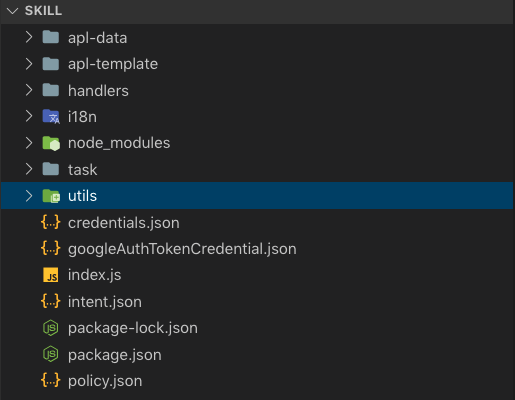
\includegraphics[width=13cm]{immagini/skill-folder.png}
	\caption{\label{fig:gerarchia_cartella_cc}Gerarchia cartella progetto C.C.}
\end{figure}

\subsection{Handlers}
Come descritto prima la cartella del progetto C.C. è stata disposta per una gestione ordinata del codice. Una delle sotto-cartelle contenute al suo interno è dedicata per la gestione degli handelrs. Nel codice della Skill gli handerls sono delle funzioni che hanno lo scopo di gestire gli intenti che vengono scatenati all'invocazione di un comando da parte dell'utente. Gli handlers sono stati così realizzati:
\begin{itemize}
    \item \texttt{index.js}: che contiene ed ingloba l'export di tutte le classi dei handlers contenuti in questa cartella
    
    \item \texttt{gestioneConsegne\_Complete.js}: questo handler ha il compito di catturare l'evento nel caso in cui l'utente intenda consegnare un pacco (o lettera) sapendo già il nome del destinatario e, o l'oggetto consegnato o la professione dell'utente che sta conversando;
    \item \texttt{gestioneConsegne\_NomeDipendete.js}: questo handler ha il compito di catturare l'evento nel caso in cui l'utente intenda consegnare un pacco (o lettera) senza sapere già il nome del destinatario. Questo gestore ha il compito di richiedere tale dato domandandolo all'utente che sta conversando con la Skill;
    \item \texttt{gestioneIncontri\_Complete.js}: questo handler ha il compito di catturare l'evento nel caso in cui l'utente visitatore abbia un appuntamento e i dati necessari sono stati tutti raccolti;
    \item \texttt{gestioneIncontri\_NomeDipendente\_NomeVisitatore.js}: questo handelr ha il compito di catturare l'evento nel caso in cui l'utente visitatore abbia un appuntamento e, il nome del dipendetene cercato e del cliente appena entrato, sono stati raccolti. Il gestore eseguirà dei controlli per verificare l'attendibilità dei dati per poi proseguire con il dialogo oppure chiedendone di nuovi dati;
    \item \texttt{gestioneIncontri\_NomeDipendente.js}: questo handler ha il compito di catturare l'evento nel caso in cui l'utente abbia un appuntamento e la Skill richiede il nome del dipendente cercato;
    \item \texttt{gestioneIncontri\_Orari.js}: questo handler ha il compito di catturare l'evento nel caso in cui l'utente abbia un appuntamento e la Skill richiede l'orario per verificare l'evento nel calendario;
    \item \texttt{vorreiIncontri\_Complete.js}: questo handler ha il compito di catturare l'evento nel caso in cui l'utente visitatore desideri incontrare un dipendente e sono stati raccolti tutti i dati necessari;
    \item \texttt{vorreiIncontri\_CompleteWithOrario.js}: questo handler ha il compito di catturare l'evento nel caso in cui l'utente visitatore desideri incontrare un dipendente e richiede l'orario di appuntamento per verificare l'esistenza dell'evento nel calendario;
    \item \texttt{vorreiIncontri\_NomeDipendente\_NomeVisitatore.js}: questo handler ha il compito di catturare l'evento nel caso in cui l'utente visitatore desideri incontrare un dipendente e, il nome del dipendetene cercato e del cliente appena entrato, sono stati raccolti. Il gestore eseguirà dei controlli per verificare l'attendibilità dei dati per poi proseguire con il dialogo oppure chiedendone di nuovi dati;
    \item \texttt{vorreiIncontri\_NomeDipendente.js}: questo handler ha il compito di catturare l'evento nel caso in cui l'utente visitatore desideri incontrare un dipendente e la Skill richiede il nome di quest'ultimo;
    \item \texttt{vorreiIncontri\_SiNo.js}: questo handler ha il compito di catturare l'evento nel caso in cui l'utente visitatore abbia un appuntamento e la Skill ne richiede l'orario per verificare l'evento nel calendario;
    \item \texttt{touchWrapperUserEvent.js}: questo handler ha il compito di catturare gli eventi scatenati dal tocco sul display.
\end{itemize}
\begin{figure}[H]
	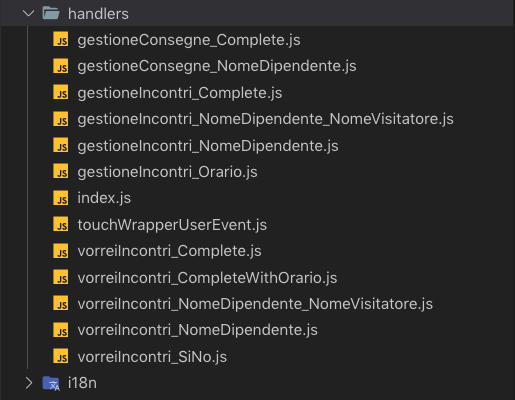
\includegraphics[width=13cm]{immagini/skill-folder2.png}
	\caption{\label{fig:gerarchia_cartella_cc2}Gerarchia cartella progetto C.C. - Handlers}
\end{figure}
\subsection{Utils}
\label{utils}
Lo stesso criterio usato per gli handlers è stato adotta anche per le classi Javascript che contengono il codice delle funzionalità della Skill. La cartella \textit{utils} contiene appunto quei metodi che permetto ad esempio la lettura del databse, l'invio di e-mail, l'invio di notifiche e la lettura del calendario. Le utilità sono state così realizzate:
\begin{itemize}
    \item \texttt{databaseUtils.js}: questa classe mette a disposizione i metodi per interrogare il database e sono presenti le seguenti funzioni:
    \begin{itemize}
        \item[>] \texttt{getInstance()}
        \item[>] \texttt{runQuery(params: var)}
        \item[>] \texttt{runScan(params: var)}
        \item[>] \texttt{runPut(params: var)}
        \item[>] \texttt{checkEmployee(nome\_dipendente: var)}
    \end{itemize}
    \item \texttt{emailUtils.js}: questa classe mette a disposizione i metodi per l'invio di messaggi e-mail ed è presente la seguente funzione:
    \begin{itemize}
        \item[>] \texttt{sendMail(from: var, to: var, message: var, oggetto: var)}
    \end{itemize}
    \item \texttt{gcalendarUtils.js}: questa classe mette a disposizione i metodi per la lettura e verifica di eventi nel calendario e sono presenti le seguenti funzioni:
    \begin{itemize}
        \item[>] \texttt{listEvents(idCalendar: var)}
        \item[>] \texttt{checkEvent(events: var, email\_dipendente: var, nome\_visitatore: var, orarioEvento: var)}
        \item[>] \texttt{generateOAuth2Client()}
    \end{itemize}
    \item \texttt{gchatUtils.js}: questa classe mette a disposizione i metodi per l'invio di notifiche su Google Chat, funzionalità in fase di sviluppo fatta nell'ultimo periodo di tirocinio, e sono presenti le seguenti funzioni:
    \begin{itemize}
        \item[>] \texttt{sendNotify(type: var, message: var)}
        \item[>] \texttt{checkThread(type: var)}
        \item[>] \texttt{putThread(thread: var, thread\_type: var)}
    \end{itemize}
    \item \texttt{prepareQuery.js}: questa classe mette a disposizioni i metodi per ricevere le query di interrogazione che si desidera e sono presenti le seguenti funzioni:
    \begin{itemize}
        \item[>] \texttt{scanEmployee()}
        \item[>] \texttt{queryEmployee(nomeDipendente: var)}
        \item[>] \texttt{putThread()}
        \item[>] \texttt{updateThread(old\_thread: var, new\_thread: var)}
    \end{itemize}
    \item \texttt{slacknotifyUtils.js}: questa classe mette a disposizione i metodi per l'invio di notifiche su Slack e al suo interno sono presenti le seguenti funzioni:
    \begin{itemize}
        \item[>] \texttt{sendNotify(channel: var, message: var)}
        \item[>] \texttt{sendDirectlyNotify(member: var, MESSAGE: var)}
        \item[>] \texttt{addTag(toTag: var)}
        \item[>] \texttt{listMembersApl(intent: var)}
        \item[>] \texttt{getIdMember(toTag: var)}
        \item[>] \texttt{membersList()}
    \end{itemize}
    \item \texttt{abracadabraUtils.js}: questo metodo contiene un easter egg\footnote{Un easter egg in informatica è un contenuto di natura bizzarra e innocuo che gli sviluppatori nascondono all'interno del prodotto}
\end{itemize}
\begin{figure}[H]
	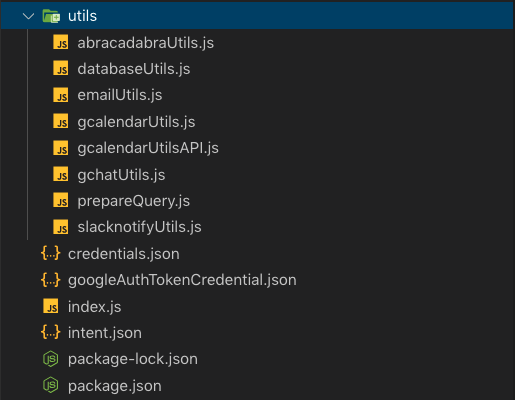
\includegraphics[width=13cm]{immagini/skill-folder3.png}
	\caption{\label{fig:gerarchia_cartella_cc3}Gerarchia cartella progetto C.C. - Utils}
\end{figure}

\section{Package utilizzati}
Particolare attenzione va fatta sulla gestione dei pacchetti e quali di essi sono stati installati nel progetto Concierge Croccante. A tale necessità è stato utilizzato il gestore di pacchetti npm, menzionato in precedente al punto \hyperref[npm]{1.5.4}, che ha consentito di installare in maniera sicura e immediata i pacchetti necessari. Installando tali pacchetti il gestore ha suddiviso il codice all'interno di una directory chiamata \texttt{node\_modules} creando inoltre un file di configurazione delle installazioni fatte.
\begin{figure}[H]
	
\includegraphics[width=12cm]{immagini/logo-npm.png}
	\caption{\label{fig:logo_npm}Logo NPM}
\end{figure}
\noindent In questa fase di progetto si è provveduto ad installare npm e tutti i pacchetti necessari alla Skill Concierge Croccante nel seguente modo:
\begin{itemize}
    \item Dalla documentazione di npm\footnote{Doc npm. URL: \href{https://docs.npmjs.com/downloading-and-installing-node-js-and-npm}{https://docs.npmjs.com/downloading-and-installing-node-js-and-npm}} viene riportato il seguente comando da eseguire su terminale:
    \begin{lstlisting}[language=bash]
		$ [sudo] npm install npm -g
	\end{lstlisting}
	Il comando installerà l'ultima versione del gestore pacchetti. Se si desidera verificare e visualizzare l'ultima versione di npm è necessario eseguire il comando: 
	\begin{lstlisting}[language=bash]
		$ npm -v
	\end{lstlisting}
	\item I pacchetti installati nel progetto sono stati i seguenti:
	\begin{itemize}
	    \item[>] \texttt{ask-sdk} e \texttt{ask-sdk-core} di AWS che semplifica la creazione di Skill, permettendo di utilizzare le funzionalità base di Alexa in maniera rapida:
	    \begin{lstlisting}[language=bash]
		    $ npm install --save ask-sdk
		    $ npm install --save ask-sdk-core
	    \end{lstlisting}
	    \item[>] \texttt{request} per semplificare ed effettuare chiamate http, supporta HTTPS i re-indirizzamenti:
	    \begin{lstlisting}[language=bash]
		    $ npm install request
	    \end{lstlisting}
	    \item[>] \texttt{googleapis} è una libreria client per l'utilizzo delle API di Google, rendendo più semplice ed immediate le chiamate ai servizi come Calendar:
	    \begin{lstlisting}[language=bash]
		    $ npm install googleapis
	    \end{lstlisting}
	    \item[>] \texttt{slack-notify} è una libreria che rende flessibile l'utilizzo dell'API Webhooks\footnote{Incoming Webhooks. URL: \href{https://api.slack.com/incoming-webhooks}{https://api.slack.com/incoming-webhooks}} di Slack, semplificando l'invio di notifiche a Slack dalla Skill:
	    \begin{lstlisting}[language=bash]
		    $ npm install slack-notify
	    \end{lstlisting}
	    \item[>] \texttt{i18next} e \texttt{i18next-sprintf-postprocessor} sono dei framework di internazionalizzazione popolari ambienti javascript:
	    \begin{lstlisting}[language=bash]
		    $ npm install i18next
		    $ npm install i18next-sprintf-postprocessor
	    \end{lstlisting}
	\end{itemize}
\end{itemize}

\newpage
\section{Calendario}
Per la soddisfazione del requisito RO17 analizzato al punto \hyperref[requisti-richiesti]{2.3}, ovvero la lettura e verifica degli appuntamenti in calendario, è stato richiesto l'uso di Google Calendar, giù utilizzato dall'azienda Crispy Bacon per le sue note funzionalità. 
\subsection{Google Calendar}
Per l’integrazione col servizio di Google Calendar sono a disposizione delle API documentate reperibili al indirizzo \href{https://developers.google.com/calendar/}{developers.google.com/calendar/}. Dalla guida emergono i seguenti requisti necessari:\\
\begin{minipage}{0.5\textwidth}
	\begin{figure}[H]
		
\includegraphics[width=5cm]{immagini/google_calendar.png}
		\caption{\label{fig:icona_google_calendar}Icona Google Calendar}
	\end{figure}
\end{minipage}
\begin{minipage}{0.5\textwidth}
	\begin{itemize}
		\item Node.js
    	\item googleapis package
    	\item Account Google funzionante e verificato
    	\item Autorizzazione OAuth\footnote{OAuth: protocollo di rete open e standard, progettato per lavorare con il protocollo HTTP.}
	\end{itemize}
\end{minipage}
\\[0.5cm]
Nei punti successivi verranno analizzati aspetti importanti, con esempi di codice, riguardante l'integrazione con il calendario in questione e l’uso delle sue API.
\subsubsection{OAuth2}
Per consentire la lettura ed ottenere la lista di eventi presenti nel calendario è stato necessario eseguire un'autenticazione tramite il protocollo OAuth 2.0\footnote{OAuth 2.0. URL: \href{https://oauth.net/2/}{https://oauth.net/2/}}. Quest'ultimo è un protocollo di rete open che consente l'emissione di un token di accesso da parte di un server autorizzato ad un client di terze parti, nel nostro caso il servizio di Google Calendar, previa approvazione dell'utente proprietario della risorsa cui si intende accedere. Per poter ottenere ciò sono stati svolti i seguenti passi:
\begin{itemize}
    \item Visitando la pagina Google Calendar API\footnote{G. Calendar API. URL: \href{https://developers.google.com/calendar/quickstart/nodejs}{https://developers.google.com/calendar/quickstart/nodejs}} è stato abilitato l'utilizzo delle API per il calendario. Nella pagina infatti è presente il primo step da seguire dal titolo ”\textit{Turn on the Google Calendar API}” dove presente il bottone adibito all'abilitazione:\\
    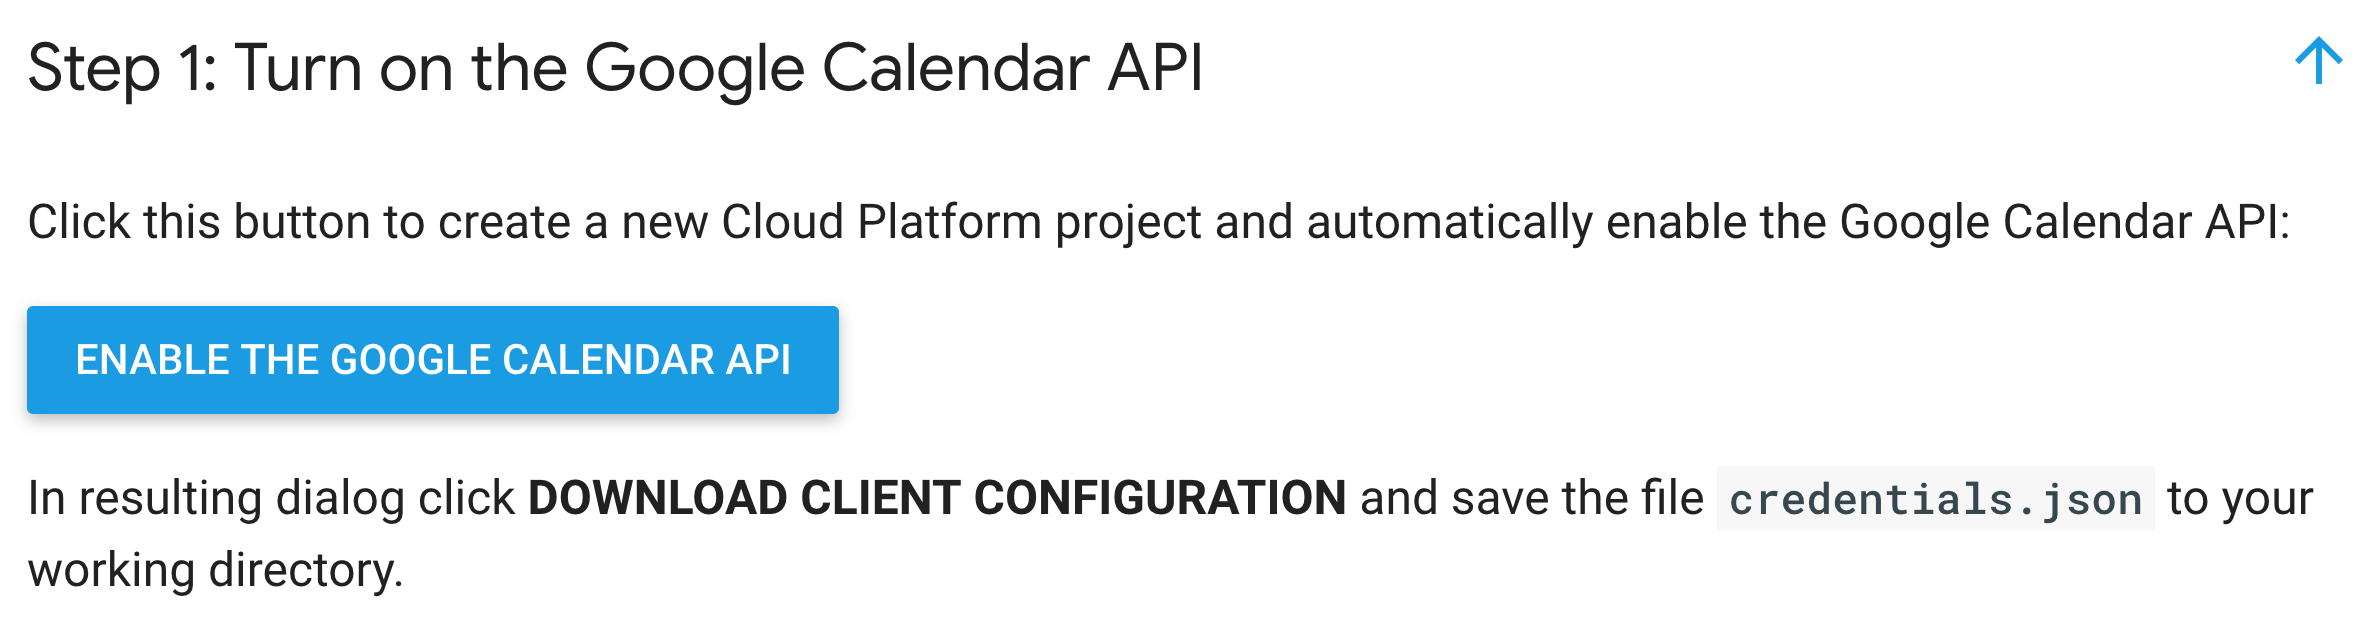
\includegraphics[width=12cm]{immagini/google_calendar_api.png}\\[2cm]
    Nella sezione corrente, una volta cliccato il bottone \texttt{ENABLE THE GOOGLE CALENDAR API} ed eseguito l’accesso con l’account Google il quale si desidera leggere gli eventi in calendario, è stato salvato il file credentials.json ottenuto dall'accesso e fornito nella cartella di progetto.
    \item Sempre nella stessa pagina è stato copiato ed eseguito l'esempio di set up riportato per ottenere l’OAuth necessario a visualizzare gli eventi nel calendario. Di seguito si riporta tale esempio di codice, importante appunto per ricevere le autorizzazioni necessarie:
	\lstinputlisting[caption=Esempio Set up Google Calendar]{code/generateGoogleAuthToken.js}
	\item Per eseguire tale esempio di codice è stato sufficiente aprire il terminale sulla cartella di progetto dove risiede il file di set up e lanciare lo script con il seguente comando:
	\begin{lstlisting}[language=bash]
		$ node [filename]
	\end{lstlisting}
	Nel caso in cui fossa la prima volta che eseguito tale esempio è necessario autorizzare l'accesso:
	\begin{enumerate}
		\item Aprire l'URL restituito dal terminale col proprio web browser
		\item Fare il login in se non si è già loggati
		\item Cliccare il bottone \texttt{Accept}
		\item Copiare il codice ricevuto, incollarlo nella terminale e premere \texttt{Enter}
	\end{enumerate}
\end{itemize}
\subsubsection{Lettura eventi}
All'interno del progetto Concierge Croccante la fase di lettura del calendario è stata semplificata realizzando una classe contenente al suo interno metodi appositi. Di tali metodi, già menzionati al punto \hyperref[utils]{3.4.2}, ne viene riportato il codice e analizzato il loro funzionamento:
\lstinputlisting[caption=Metodi listEvent e generateOAuth2Client]{code/gcalendarUtils1.js}
Per ottenere la lista di eventi non servirà altro che richiamare \texttt{listEvents(idCalendar)}. La funzione ritornerà un oggetto contenente tutti gli eventi, con le loro informazioni, della giornata odierna fino ad un massimo di 15 risultato. Attenzione: i file citati credentials.json e googleAuthTokenCredential.json non sono altro che le credenziali recuperate nei punti precedenti per accedere con il token OAuth.
\\[0.5cm]
Altro metodo presente e largamente utilizzato è \texttt{checkEvent(events, email\_dipendente, nome\_visitatore, orarioEvento)}:
\lstinputlisting[caption=Metodo checkEvent]{code/gcalendarUtils2.js}
Questo metodo pone come precondizione il fatto di ricevere in ingresso l'elenco di eventi ed i valori: nome visitatore, nome persona cercata ed orario; non vuoti. Il risultato sarà un valore \textit{boolean false} nel caso \textbf{non} sia presente alcun evento nel calendario, un valore numerico \textit{1} nel caso sia stato trovato un evento per la persona e l'orario indicato, oppure \textit{0} se esiste un evento ma l'orario indicato non coincide con quello effettivo.

\newpage
\section{Invio notifiche}
Altra specifica per la soddisfazione dei requisiti RO18 e RO19 analizzati al punto \hyperref[requisti-richiesti]{2.3}, è l'invio di notifiche. Per ovviare a ciò sono state realizzate le funzionalità per l'invio di messaggi istantanei via Slack e e-mail via AWS SES visto il già utilizzo di questi servizi da parte di Crispy Bacon.
\subsection{Slack}
Per l’integrazione col servizio di Slack sono a disposizione delle API documentate reperibili al indirizzo \href{https://api.slack.com/}{api.slack.com/}. Dalla guida emergono i seguenti requisti necessari:
\\
\begin{minipage}{0.5\textwidth}
	\begin{figure}[H]
		
\includegraphics[width=6cm]{immagini/slack.png}
		\caption{\label{fig:icona_slack}Icona servizio - Slack}
	\end{figure}
\end{minipage}
\begin{minipage}{0.5\textwidth}
	\begin{itemize}
		\item Node.js
		\item slack-notify package
		\item Account Slack
		\item Incoming Webhook
	\end{itemize}
\end{minipage}
\\[0.4cm]
Nei punti successivi verranno analizzati aspetti importanti, con esempi di codice, riguardante l'invio di notifiche con Slack e l’uso delle sue API.
\subsubsection{Incoming Webhooks}
Per consentire l'invio di messaggi di notifica via chat viene scelto di utilizzare un bot con Incoming Webhook\footnote{\href{https://it.wikipedia.org/wiki/Webhook}{https://it.wikipedia.org/wiki/Webhook}}. Quest'ultimo è un mezzo con il quale si semplifica l'invio di messaggi da un'applicazione a Slack. La creazione di un Incoming Webhook fornisce un URL univoco a cui si invia un payload JSON con il testo del messaggio e alcune opzioni.
Per ottenere l'Incoming Webhook sono stati eseguiti i seguenti passaggi:
\begin{itemize}
    \item Visitando la pagina dedicata \href{https://api.slack.com/incoming-webhooks}{api.slack.com/incoming-webhooks} è stata creata un'App per Slack cliccando sul bottone \texttt{"Create your Slack app"}:\\
    
\includegraphics[width=12cm]{immagini/slack_bot.png}\\
    Si viene successivamente indirizzati in una nuova pagina dove sarà possibile creare la propria App per Slack:
	\begin{enumerate}
		\item Cliccare sul bottone \texttt{Create New App}
		\item Inserire il nome dell'app
		\item Scegliere lo \textit{space} di lavoro dove installare l'app
		\item Cliccare su \texttt{Crea App}
	\end{enumerate}
	\item Dopo aver creato l'App è stato abilitato l'Incoming Webhook nell'apposita pagina delle impostazioni. Fatto sono state visualizzate alcune opzioni aggiuntive. Tra queste era presente il pulsante \textit{Aggiungi nuovo Webhook a Workspace}. Viene quindi aggiunto il Webhook ad canale/space di Slack designato per pubblicare l'App e salvata tale modifica facendo clic su \texttt{Autorizza la tua app}.
\end{itemize} 
\subsubsection{Invio messaggi}
All'interno del progetto Concierge Croccante la fase di notifica via Slack è stata semplificata realizzando una classe contenente al suo interno metodi appositi. Di tali metodi menzionati al punto \hyperref[utils]{3.4.2} ne viene riportato il codice e analizzato il loro funzionamento\footnote{NB: la variabile \texttt{MY SLACK WEBHOOK URL} contiene l'URL del Webhook dell'App}: 
\lstinputlisting[caption=Metodo sendNotify]{code/slacknotifyUtils1.js}
Il codice sopra riportato mostra il metodo \texttt{sendNotify(channel:  var, message:  var)}: tale funzione non fa altro che inviare il testo del messaggio nel canale di Slack desiderato passando i dati per parametro. La variabile constante \texttt{slack.send} richiama il metodo fornito del pacchetto \texttt{slack-notify} che non farà altro che fare una \textit{request} in \textit{POST} all'API \texttt{chat.postMessage}. Nel caso in cui il metodo riscontrasse un errore nell'invio del messaggio viene lanciata un eccezione.

\newpage
\lstinputlisting[caption=Metodo sendDirectlyNotify]{code/slacknotifyUtils2.js}
Per l'invio delle notifiche in direct message\footnote{Messaggio privato inviato in un social media} è stato messo a disposizione il metodo \texttt{sendDirectlyNotify(member:  var, MESSAGE:  var)}: tale funzione invierà il testo del messaggio al destinatario indicato alla funzione facendo, anche in questo caso, una \textit{request} in \textit{POST} all'API \texttt{chat.postMessage}. Differentemente dal metodo precedente qui non viene utilizzata alcuna libreria, ma viene usata l'API in maniera diretta.

\newpage
\lstinputlisting[caption=Metodo addTag]{code/slacknotifyUtils3.js}
Altra funzionalità messa a disposizione dalla classe è il metodo \texttt{addTag(toTag: var)}: tale funzione non fa altro che richiamare una funzione ausiliaria e privata della classe, più elaborata e non visibile all'utente esterno, che va ad aggiungere, grazie all'id del membro cercato, il tag necessario per menzionarlo all'interno delle chat di gruppo.

\newpage
\lstinputlisting[caption=Metodo listMembersApl]{code/slacknotifyUtils4.js}
Metodo più rilevante è \texttt{listMembersApl(intent: var)}: tale metodo viene richiamato dalla Skill qualora è necessaria la costruzione di un APL con elementi touch che al momento del tocco scatenino un evento. In questo caso l'APL che si va a creare è una lista dei membri di Crispy Bacon dove è possibile selezionare il nome per fornirlo alla Skill. 

\newpage
\subsection{E-mail}
Per l'invio di notifiche via e-mail, come già detto in precedenza, è stato utilizzato il servizio Amazon SES e la sua integrazione con il servizio sono necessari i seguenti requisiti:
\\
\begin{minipage}{0.47\textwidth}
	\begin{figure}[H]
		
\includegraphics[width=6cm]{immagini/ses.png}
		\caption{\label{fig:google_calendar}Icona servizio - SES}
	\end{figure}
\end{minipage}
\begin{minipage}{0.5\textwidth}
	\begin{itemize}
		\item Node.js
		\item npm aws-sdk
		\item Account AWS
		\item Indirizzo e-mail
	\end{itemize}
\end{minipage}
\\[0.4cm]
Nei punti successivi verranno analizzati aspetti importanti, con esempi di codice, riguardante l'invio di e-mail con Amazon SES e l'uso della libreria SDK.

\subsubsection{Invio e-mail}
All'interno del progetto Concierge Croccante l'invio di notifiche o messaggi via e-mail è stata semplificata realizzando una classe contenente al suo interno metodi appositi. Di tali metodi menzionati al punto \hyperref[utils]{3.4.2} ne viene riportato il codice e analizzato il loro funzionamento: 

\lstinputlisting[caption=Metodo sendMail]{code/emailUtils.js}
Il codice sopra riportato mostra il metodo \texttt{sendMail(from:  var, to:  var, message:  var, oggetto:  var)}: tale funzione non fa altro che inviare una e-mail con i campi from, to, message ed oggeto passati per parametro. La variabile constante \texttt{ses} non fa altro che richiamare il metodo fornito del pacchetto \texttt{aws-sdk} che si occuperà di richiamare le API necessarie all'utilizzo di AWS SES.

\newpage
\section{Lettura del Database}
Funzionalità a supporto di quelle principali è la lettura del database DynamoDB. Quest'ultimo è popolato da una tabella contente i nomi di tutti i dipendenti dell'azienda Crispy Bacon, i quali, vengono prelevati per essere utilizzati nelle fasi di controllo, come la ricerca di un dipendente per verificarne la sua esistenza. Il progetto predispone due classi adibite a questo tipo di funzionalità per interrogare il database: \texttt{databaseUtils.js} e \texttt{prepareQuery.js}.

\lstinputlisting[caption=Metodo getInstance e runQuery]{code/databaseUtils.js}
Il codice sopra riportato mostra la classe coi metodi per eseguire \textit{query} di diversa tipologia: \texttt{runQuery(params:  var)} non fa altro che richiamare il metodo presente nel pacchetto \texttt{aws-sdk} per l'esecuzione di un interrogazione standard. Altri metodi come \texttt{runScan(params:  var)} e \texttt{runPut(params:  var)} eseguono una scansione e un inserimento nel database secondo i parametri\footnote{La classe \texttt{prepareQuery.js} svolge perll'appunto questo ruolo. I metodi della classe ritornano un oggetto contente i parametri necessari per l'esecuzione della query desiderata} passati alle funzioni.

\newpage
\section{Async e Await}
Nella la fase di stesura del codice durante il periodo di tirocinio è stato affrontato e studiato il tema della chiamate asincrone: Async/await functions. Questo modello di funzioni va inserito nel contesto delle \textit{Promise} che, come suggerisce il suo nome, restituisce un risultato nel futuro che può essere di tipo \textit{resolve}, nel caso di successo nell'azione svolta, o \textit{reject} nel caso di un fallimento con conseguenza di errore. Per fare ciò la sintassi async/await permette di lavorare con le \textit{Promise} in un modo più confortevole e facile da usare. Per spiegare il significato di questa sintassi vengono fatti i seguenti esempi estratti dal codice della Skill Concierge Croccante. Il seguente esempio mostra una funzione che ritorna una promessa, ovvero un risultato dopo aver eseguito determinati calcoli. In questo caso ritorna una Promise con \textit{resolve} nel caso di un risultato da parte della chiamata API:
\lstinputlisting[caption=Esempio codice con Promise]{code/promise.js}
\noindent Si necessita ora che la funzione chiamante il metodo \texttt{getIdMember(toTag: var)} attenda il risultato della \textit{Promise} prima di proseguire con le istruzioni successive. Il modello async/await risolve tale necessità: dichiarando la funzione principale async e mettendo la keyword await davanti alla chiamata del metodo \texttt{getIdMember(toTag: var)} si attenderà il risultato ritornato da quest'ultima.
\lstinputlisting[caption=Esempio codice con Promise]{code/async_await.js}

\newpage
\section{Verifica e validazione}
\label{cap:verifica_validazione}
%**************************************************************
Ultima fase del periodo di tirocinio è stato svolto dal processo di verifica e validazione. La prima è un processo che si occupa di fornire evidenza oggettiva, ovvero che i risultati ottenuti come output dello sviluppo del software soddisfino i requisiti, la seconda invece è un processo per confermare in modo definitivo che le caratteristiche del software siano conformi ai bisogni dell'utente e all'uso previsto.
Per eseguire la verifica e la validazione è necessario l'esecuzione di test\footnote{In ambito informatico i test eseguiti nel processo di verifica sono eseguiti in maniera automatica durante lo sviluppo del software} che individuino carenze, correttezza e affidabilità. Nel progetto della Skill Concierge Croccante non è stato realizzato alcun test per il processo di verifica: viste le tempisti non è stato ritenuto necessario e si è pertanto scelto di eseguire test già esistenti nel servizio Amazon Lambda, sufficienti ad esaminare il codice e rilevare eventuali errori. Per quanto riguarda il processo di validazione\footnote{Attività di supporto la quale accerta che il prodotto dei processi rispetti le specifiche} è stato svolto, alla fine del periodo di tirocinio, un incontro  con il tutor aziendale e CFO Damiano Buscemi come conferma fiale la quale ha accertato le bontà richieste dal prodotto finale. Tale validazione non è stata altro che una dimostrazione funzionante della Skill, eseguita prima da me per spiegare spiegare le varie funzionalità, ed infine da Crispy Bacon come conferma.
\\[0.5cm]
\noindent Per quanto riguarda l'integrazione coi servizi utilizzati, nello specifico Google Calendar e Slack, sono stati creati dei file appositi da eseguire manualmente che verificano il corretto funzionamento di essi restituendo un risultato:
\begin{figure}[H]
	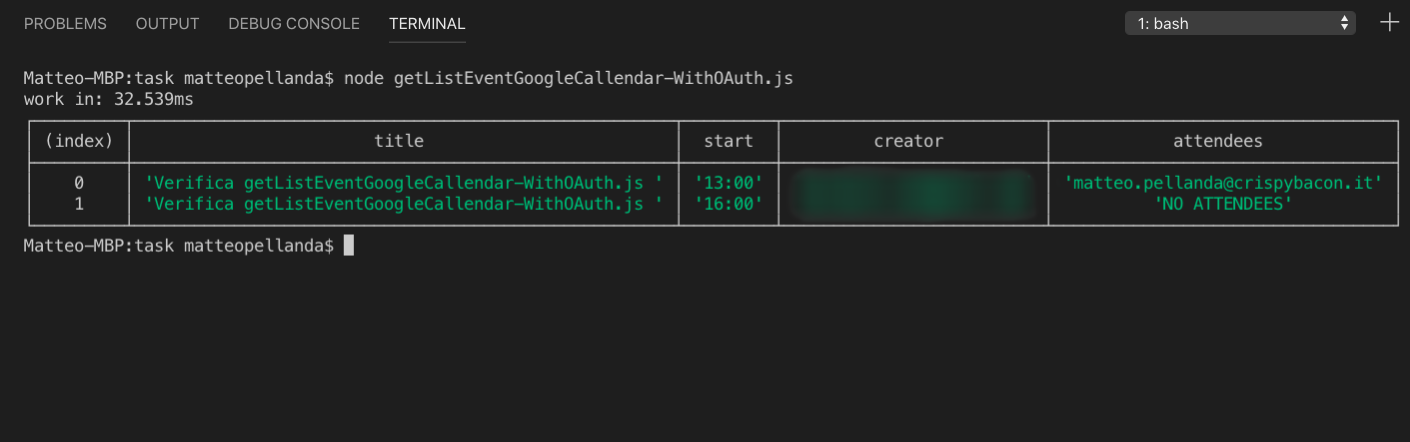
\includegraphics[width=13cm]{immagini/test-googleCalendar.png}
	\caption{\label{fig:test_googleCalendar}Esempio test funzionamento Google Calendar - Lista eventi}
\end{figure}
\newpage
\noindent L'immagine mostra l'esecuzione del file getListEventGoogleCallendar-WithOAuth.js adibito a verificare la validità del token OAuth per ottenere la lista di eventi della giornata corrente. Inoltre verifica la corretta chiamata dell'API \texttt{calendar.events.list}.
\begin{figure}[H]
	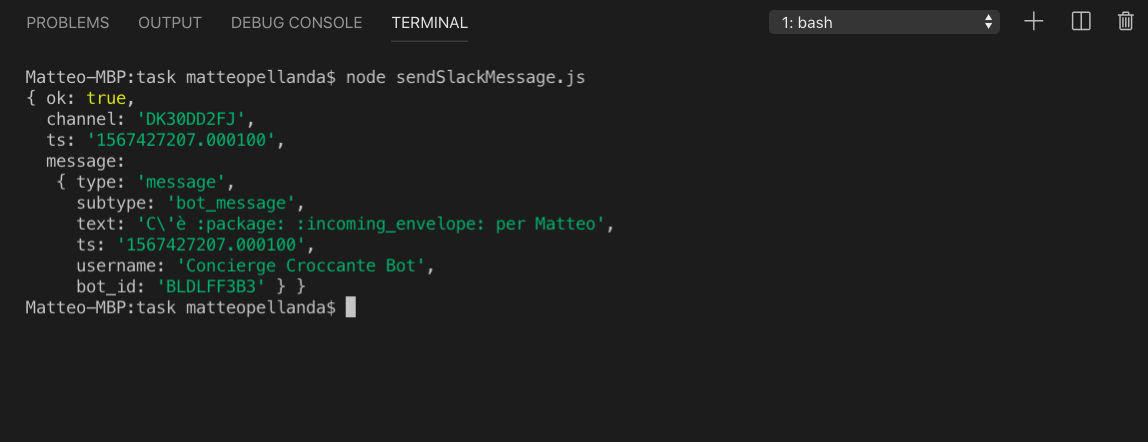
\includegraphics[width=13cm]{immagini/test-sendSlack.png}
	\caption{\label{fig:test_slack_send}Esempio test funzionamento Slack - Invio messaggio}
\end{figure}
\noindent L'immagine mostra l'esecuzione del file sendSlackMessage.js adibito a verificare la validità del token per inviare messaggi di notifica via Slack. Inoltre verifica la corretta chiamata dell'API \texttt{chat.postMessage}.
\begin{figure}[H]
	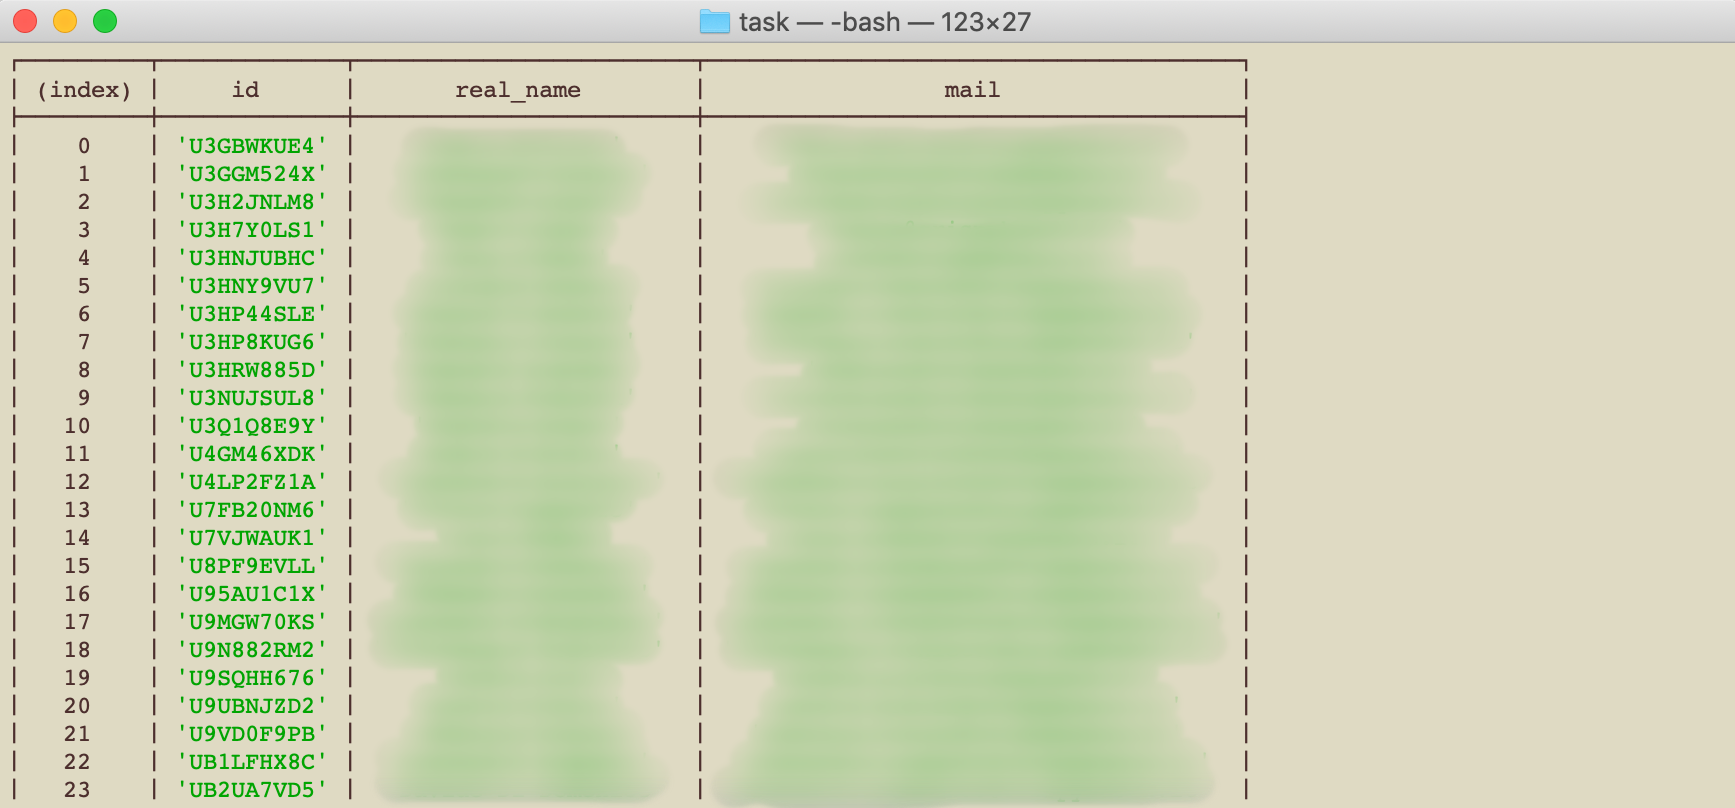
\includegraphics[width=13cm]{immagini/test-listSlack.png}
	\caption{\label{fig:test_slack_list}Esempio test funzionamento Slack - Lista membri}
\end{figure}
\noindent L'immagine mostra l'esecuzione del file getSlackListMemebers.js adibito a verificare la validità del token per ottenere la lista dei membri di Crispy Bacon. Inoltre verifica la corretta chiamata dell'API \texttt{users.list}.


